\documentclass[10pt,twocolumn,letterpaper]{article}

% ---------- Fonts & Encoding ----------
\usepackage[utf8]{inputenc}
\usepackage[T1]{fontenc}
\usepackage{libertine}
\usepackage{libertineMono}

% ---------- Page Layout ----------
\usepackage[margin=0.85in,columnsep=0.3in]{geometry}
\usepackage{parskip}
\setlength{\parskip}{4pt plus 1pt minus 1pt}

% ---------- Section Formatting ----------
\usepackage{titlesec}
\titleformat{\section}{\large\bfseries\sffamily}{\thesection}{0.8em}{}
\titleformat{\subsection}{\normalsize\bfseries\sffamily}{\thesubsection}{0.7em}{}
\titleformat{\subsubsection}{\normalsize\itshape\sffamily}{\thesubsubsection}{0.6em}{}
\titlespacing*{\section}{0pt}{14pt plus 2pt}{6pt plus 1pt}
\titlespacing*{\subsection}{0pt}{10pt plus 2pt}{4pt plus 1pt}
\titlespacing*{\subsubsection}{0pt}{8pt plus 2pt}{3pt plus 1pt}

% ---------- Math & Theorems ----------
\usepackage{amsmath}
\let\Bbbk\relax
\usepackage{amssymb}
\let\openbox\relax
\usepackage{amsthm}
\newtheorem{theorem}{Theorem}
\newtheorem{definition}{Definition}
\newtheorem{corollary}{Corollary}
\newtheorem{lemma}{Lemma}
\newtheorem{proposition}{Proposition}

% ---------- Tables ----------
\usepackage{booktabs}
\usepackage{tabularx}
\renewcommand{\arraystretch}{1.15}

% ---------- Figures & Graphics ----------
\usepackage{graphicx}
\usepackage{tikz}
\usetikzlibrary{positioning,arrows.meta,shapes.geometric,fit,backgrounds,calc}
\usepackage{caption}
\captionsetup{font=small,labelfont=bf,skip=6pt}

% ---------- Code Listings ----------
\usepackage{listings}
\usepackage{xcolor}
\definecolor{codebg}{HTML}{F7F7F8}
\definecolor{codeframe}{HTML}{E0E0E0}
\definecolor{kw}{HTML}{1A5276}
\definecolor{cmt}{HTML}{6C7A89}
\lstdefinestyle{code}{
    basicstyle=\ttfamily\footnotesize,
    breaklines=true,
    frame=single,
    framesep=6pt,
    xleftmargin=6pt,
    xrightmargin=2pt,
    backgroundcolor=\color{codebg},
    rulecolor=\color{codeframe},
    keywordstyle=\color{kw}\bfseries,
    commentstyle=\color{cmt}\itshape,
    numbers=none,
    captionpos=b,
    aboveskip=8pt,
    belowskip=8pt,
}
\lstset{style=code}

% ---------- Hyperlinks ----------
\usepackage[colorlinks=true,linkcolor=blue!50!black,citecolor=blue!50!black,urlcolor=blue!50!black]{hyperref}
\usepackage{url}
\usepackage{enumitem}

% ---------- Header ----------
\usepackage{fancyhdr}
\pagestyle{fancy}
\fancyhf{}
\renewcommand{\headrulewidth}{0.4pt}
\fancyhead[L]{\small\sffamily Private Decentralized Inference on Consumer Hardware}
\fancyhead[R]{\small\sffamily\thepage}
\fancyfoot{}

% =====================================================================
\title{%
\vspace{-0.5cm}
{\LARGE\sffamily\bfseries Private Decentralized Inference\\on Consumer Hardware}\\[8pt]
{\large\sffamily Enabling Confidential Computation on Third-Party Apple Silicon\\via Software Access Path Elimination}
}

\author{
    \textbf{Gajesh Naik} \\[4pt]
    {\small Eigen Labs} \\[2pt]
    {\small\texttt{gajesh@eigenlabs.org}}
}

\date{\small April 2026}

% =====================================================================
\begin{document}

\twocolumn[
\maketitle
\thispagestyle{fancy}

% ---------- Abstract ----------
\begin{@twocolumnfalse}
\begin{abstract}
\noindent
We present a system and method for private machine learning inference on a decentralized network of consumer hardware. The core problem: a user wants to run an AI model on someone else's Mac, but the machine's owner---who has root access and physical custody---should not be able to see the user's prompts or the model's responses. The machines lack hardware Trusted Execution Environments (TEEs) for application-level memory isolation.

Our approach eliminates every software path through which inference data could be observed. The inference engine runs directly inside a single hardened process---no subprocess, no local server, no inter-process communication. The macOS kernel blocks all external access to this process's memory: debuggers are denied at the system call level (\texttt{PT\_DENY\_ATTACH}), memory-reading APIs are blocked by Hardened Runtime, and these protections cannot be disabled without rebooting, which terminates the process and erases its data. We prove that System Integrity Protection, once verified, is immutable for the process lifetime (Theorem~\ref{thm:sip}).

A multi-layer attestation architecture verifies each machine in the network: (1)~a Secure Enclave signature proves hardware-bound identity, (2)~Apple's MDM framework independently confirms the machine's security configuration, (3)~Apple's Managed Device Attestation (MDA) produces an Apple-signed certificate chain proving the device is genuine hardware, with an MDA nonce binding the provider's signing key to the attested device, and (4)~periodic challenge-response confirms security posture has not degraded since enrollment.

After eliminating all software access paths, the only remaining attack requires physically probing the memory chips---which are soldered directly into Apple's System-on-Chip package. This is the same residual threat model accepted by Apple's Private Cloud Compute~\cite{apple-pcc} for Siri and Apple Intelligence. We validate the system end-to-end on production hardware with live inference, demonstrating negligible security overhead (12\,ms per request).
\end{abstract}
\vspace{16pt}
\end{@twocolumnfalse}
]

% =====================================================================
\section{Introduction}
\label{sec:intro}

When a user sends a prompt to a cloud AI service, that prompt travels to a server owned and operated by someone else. The user's privacy rests on a contractual promise---a privacy policy---not a technical guarantee. Hardware Trusted Execution Environments (TEEs) such as Intel TDX~\cite{intel-tdx}, AMD SEV-SNP~\cite{amd-sev}, and NVIDIA Confidential Computing~\cite{nvidia-cc} can provide cryptographic memory isolation, but these technologies exist only on enterprise server hardware costing \$14,000 or more.

Meanwhile, over 100 million Apple Silicon Macs have been sold since 2020. With 64--256\,GB of unified memory and 273--819\,GB/s memory bandwidth, they can run models with up to 235 billion parameters at interactive speeds. These machines sit idle most of the day. A decentralized network that lets Mac owners contribute their idle compute for AI inference---while guaranteeing that they cannot see the prompts being processed---would make private inference available at a fraction of the cost of cloud TEEs.

The challenge is that Apple Silicon provides no hardware TEE accessible to third-party applications:

\begin{itemize}[leftmargin=*,itemsep=2pt,topsep=2pt]
    \item The \textbf{Secure Enclave} provides hardware-bound P-256 key generation and ECDSA signing, but cannot encrypt main system memory or provide isolated execution for arbitrary code.
    \item \textbf{App Attest} (\texttt{DCAppAttestService}) returns \texttt{false} for \texttt{isSupported} on macOS---it is available only on iOS and iPadOS.
    \item No public API exposes boot measurements or PCR-style remote attestation.
\end{itemize}

We present a system that makes this possible. Rather than encrypting memory (which Apple Silicon cannot do for third-party code), we \emph{eliminate every software mechanism} through which the machine's owner could observe inference data---the same design philosophy Apple employs in Private Cloud Compute~\cite{apple-pcc}. Apple's PCC removes all software interfaces (shell, debugger, persistent storage) that could access inference data. We apply this principle to a harder problem: in PCC, Apple owns the hardware and controls physical access; in our system, the hardware owner is the adversary.

\textbf{Contributions.} This paper makes the following contributions:
\begin{enumerate}[leftmargin=*,itemsep=2pt,topsep=2pt]
    \item A \textbf{decentralized private inference architecture} that enables confidential AI computation on a network of third-party Apple Silicon machines, where each machine's owner is assumed to be adversarial.
    \item A \textbf{formal security model} for this setting, including a proof that System Integrity Protection provides runtime immutability under standard assumptions (Theorem~\ref{thm:sip}), and a complete enumeration of the software attack surface.
    \item An \textbf{in-process inference design} that embeds the inference engine directly in a hardened process, eliminating all inter-process communication channels that could be observed, with optional \textbf{hypervisor memory isolation} that extends protection from software-enforced to hardware-enforced via ARM Stage~2 page tables at zero performance cost.
    \item A \textbf{multi-layer attestation architecture} combining Secure Enclave signatures, MDM-based independent verification, Apple MDA hardware attestation with Apple-signed certificate chains, MDA nonce-based SE key binding, and periodic challenge-response with fresh security state.
    \item A \textbf{combined enrollment protocol} that unifies MDM enrollment and ACME device attestation into a single configuration profile, reducing trust establishment to a one-step process.
    \item \textbf{End-to-end validation} on production hardware (Apple M2 and M4~Max) with live inference, demonstrating that the security mechanisms introduce negligible overhead.
    \item A \textbf{cost analysis} showing that Mixture-of-Experts models create 6--32$\times$ cost advantages on unified-memory hardware versus cloud GPUs, establishing economic feasibility.
\end{enumerate}

% =====================================================================
\section{Related Work}
\label{sec:related}

\textbf{Hardware TEE-based inference.}\quad Intel TDX~\cite{intel-tdx} and AMD SEV-SNP~\cite{amd-sev} encrypt VM memory and provide remote attestation. NVIDIA Confidential Computing~\cite{nvidia-cc} extends this to GPU memory. These approaches provide strong isolation but require enterprise server hardware. Our work achieves comparable privacy guarantees on consumer hardware without memory encryption.

\textbf{Decentralized compute networks.}\quad Akash~\cite{akash} provides general compute with TEE support in development. io.net~\cite{ionet} aggregates GPU resources without hardware security guarantees. Ritual~\cite{ritual} uses zero-knowledge proofs and Intel SGX. Bittensor~\cite{bittensor} employs stake-weighted consensus for result verification. None address inference privacy on consumer hardware lacking TEEs.

\textbf{Apple Private Cloud Compute.}\quad PCC~\cite{apple-pcc} achieves inference privacy on Apple Silicon servers (M2~Ultra) without memory encryption through five requirements: stateless computation, enforceable guarantees, no privileged runtime access, non-targetability, and verifiable transparency. Implementation includes: no persistent storage, no SSH or shell access, immutable OS via Signed System Volume, cryptographic erasure on reboot, and OHTTP anonymization. Our work differs in that PCC operates in \emph{Apple-controlled data centers} with physical security (access controls, tamper detection), while our system must defend against the hardware owner as adversary.

\textbf{Cryptographic approaches.}\quad Fully Homomorphic Encryption~\cite{gentry-fhe} introduces $10^4$--$10^6\times$ computational overhead. Secure Multi-Party Computation~\cite{yao-mpc} requires multiple non-colluding servers. zkLLM~\cite{zkllm} and DeepProve-1~\cite{deepprove} verify inference integrity via zero-knowledge proofs but do not protect input privacy during computation. These remain impractical for interactive LLM inference at current performance levels.

% =====================================================================
\section{Threat Model and Assumptions}
\label{sec:threat}

The fundamental challenge in decentralized inference is that the person running the computation is not the person who owns the data. A provider contributes their Mac's compute, but should learn nothing about the prompts processed on it. This section formalizes what we assume about each party and what a malicious provider can attempt.

\subsection{Actors}

\begin{definition}[System Actors]
\label{def:actors}
We define four classes of actor:
\begin{itemize}[leftmargin=*,itemsep=1pt,topsep=2pt]
    \item $\mathcal{C}$ (Consumer): The party submitting inference requests. Trusted---they have no incentive to attack their own data.
    \item $\mathcal{K}$ (Coordinator): The routing and verification service. Trusted via hardware: runs on Intel TDX~\cite{intel-tdx} with cryptographic attestation of the deployed container image. The coordinator's memory is encrypted by the TEE hardware; neither the cloud operator nor the system operator can access it.
    \item $\mathcal{P}$ (Provider): The Mac owner contributing compute. \textbf{Assumed adversarial}---they own the hardware, have root access, and may actively attempt to read inference data. This is the strongest practical assumption: we guarantee privacy even if the provider is trying to break it.
    \item $\mathcal{A}$ (Apple): Trusted for the correctness of Secure Enclave hardware, SIP implementation, Kernel Integrity Protection, Hardened Runtime enforcement, IOMMU policy, code signature verification, and the Managed Device Attestation certificate authority.
\end{itemize}
\end{definition}

\subsection{Adversary Capabilities}

\begin{definition}[Threat Model]
\label{def:threat}
The adversarial provider $\mathcal{P}$ can:
\begin{itemize}[leftmargin=*,itemsep=1pt]
    \item Execute arbitrary code as root on the Mac
    \item Install any user-level software (subject to SIP restrictions)
    \item Reboot the machine at any time
    \item Physically access the machine exterior and ports
    \item Enable RDMA over Thunderbolt~5 (requires Recovery OS boot)
    \item Attempt to intercept or modify network traffic
\end{itemize}
The adversary $\mathcal{P}$ \emph{cannot}:
\begin{itemize}[leftmargin=*,itemsep=1pt]
    \item Exploit unpatched kernel vulnerabilities (Assumption~\ref{asm:kernel})
    \item Modify Secure Enclave firmware or extract its keys
    \item Desolder LPDDR5x memory from the SoC package without destroying it
    \item Compromise Apple's Managed Device Attestation signing infrastructure
\end{itemize}
\end{definition}

\begin{definition}[Assumptions]
\label{asm:kernel}
\textbf{Assumption 1} (Kernel Integrity): The macOS kernel has no unpatched vulnerabilities that allow SIP bypass, Hardened Runtime bypass, or KIP circumvention. Apple has patched all known SIP bypass CVEs (e.g., CVE-2022-22583, CVE-2022-42821, CVE-2023-32369) within weeks of disclosure.

\textbf{Assumption 2} (Secure Enclave Integrity): The Secure Enclave hardware and firmware correctly implement key generation, signing, and key isolation. This is analogous to trusting Intel SGX or ARM TrustZone hardware.

\textbf{Assumption 3} (Apple Attestation CA Integrity): Apple's Enterprise Attestation Root CA private key is not compromised, and Apple's attestation servers correctly verify device properties before issuing certificates. This is analogous to trusting any certificate authority in the Web PKI.
\end{definition}

\subsection{Security Goal}

In plain terms: a provider processes a prompt on their Mac, returns the result, and learns nothing about what the prompt said or what the model replied. More precisely:

\begin{definition}[Privacy Property]
\label{def:privacy}
Let $x$ be an inference input (prompt) and $y = f(x)$ the model output. The system satisfies the \emph{privacy property} if, for all polynomial-time adversaries $\mathcal{P}$:
\begin{equation}
\Pr[\mathcal{P} \text{ learns } x \text{ or } y] \leq \text{negl}(\lambda)
\end{equation}
where $\lambda$ is the security parameter, under Assumptions 1--3, excluding physical memory probing attacks requiring destructive hardware modification.
\end{definition}

% =====================================================================
\section{System Architecture}
\label{sec:arch}

The decentralized network comprises three principal components: a \emph{coordinator} that routes consumer requests to providers and verifies their attestations, \emph{provider agents} running on Apple Silicon Macs that execute inference, and a \emph{Secure Enclave module} that gives each provider a hardware-bound cryptographic identity. Figure~\ref{fig:arch} depicts the complete architecture.

\begin{figure*}[t]
\centering
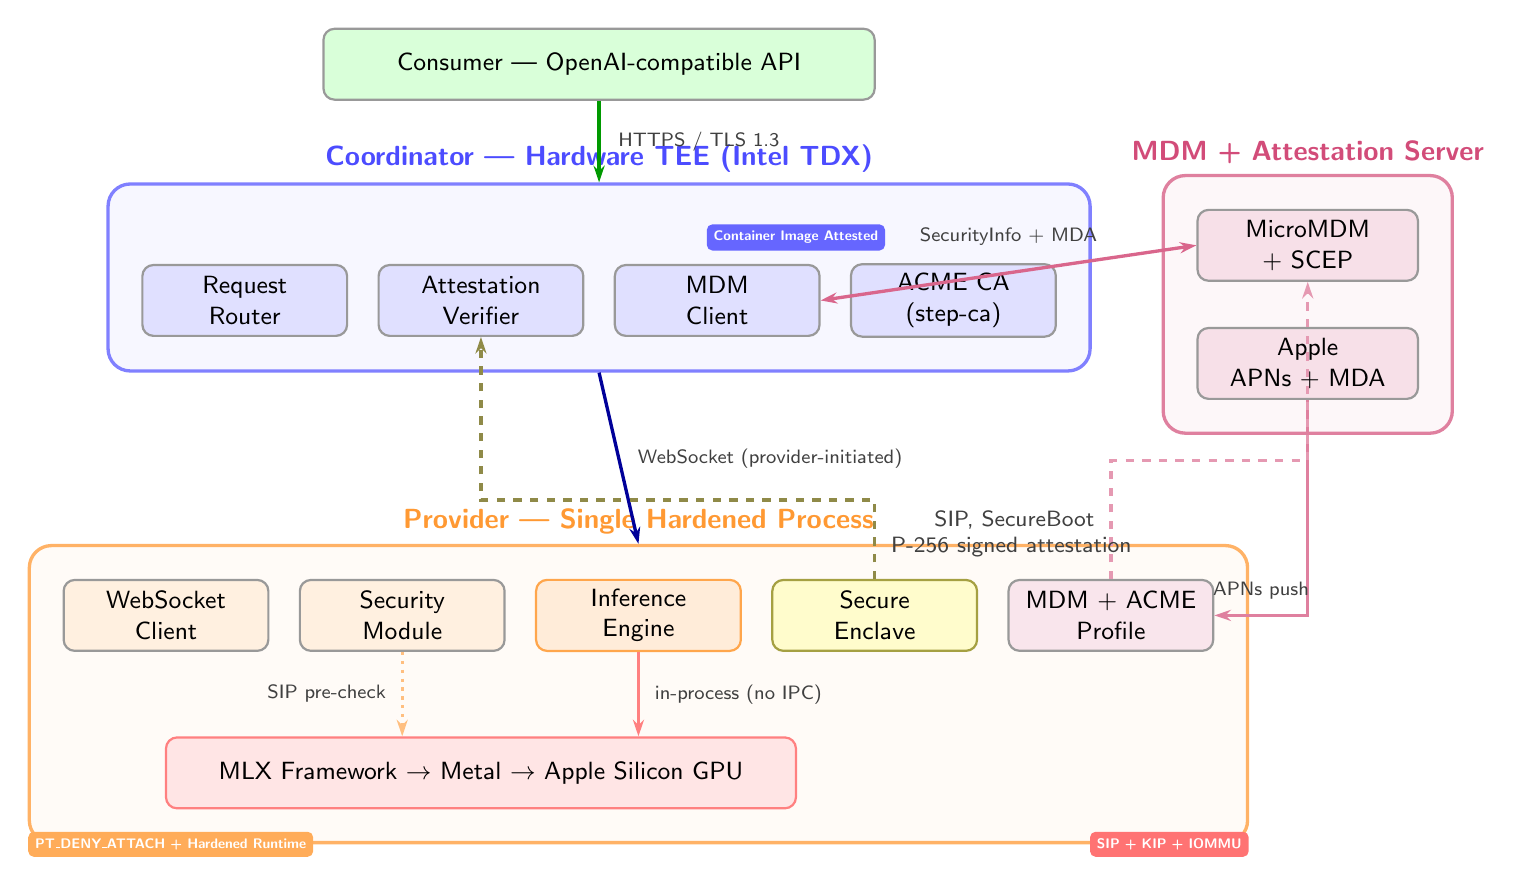
\begin{tikzpicture}[
    component/.style={draw=gray!80, thick, rounded corners=4pt, fill=#1, minimum width=2.6cm, minimum height=0.9cm, font=\small\sffamily, align=center},
    component/.default={white},
    groupbox/.style={draw=#1, very thick, rounded corners=8pt, inner sep=12pt},
    groupbox/.default={gray!50},
    arr/.style={-{Stealth[length=6pt,width=4pt]}, very thick, #1},
    arr/.default={gray!60},
    biarr/.style={{Stealth[length=6pt,width=4pt]}-{Stealth[length=6pt,width=4pt]}, very thick, #1},
    biarr/.default={gray!60},
    lbl/.style={font=\scriptsize\sffamily, #1},
    lbl/.default={gray!50!black},
    grouptitle/.style={font=\normalsize\sffamily\bfseries, #1},
    grouptitle/.default={black},
    badge/.style={font=\tiny\sffamily\bfseries, rounded corners=2pt, fill=#1, text=white, inner sep=2.5pt},
]

\node[component=green!15, minimum width=7cm] (consumer) at (0, 0) {Consumer --- OpenAI-compatible API};

\node[component=blue!12] (router) at (-4.5, -3) {Request\\Router};
\node[component=blue!12] (attverify) at (-1.5, -3) {Attestation\\Verifier};
\node[component=blue!12] (mdmclient) at (1.5, -3) {MDM\\Client};
\node[component=blue!12] (acmeca) at (4.5, -3) {ACME CA\\(step-ca)};
\node[minimum height=0.5cm, minimum width=1cm] (coordspacer) at (4.5, -2.2) {};
\begin{scope}[on background layer]
\node[groupbox=blue!50, fill=blue!3, fit=(router)(attverify)(mdmclient)(acmeca)(coordspacer),
      label={[grouptitle=blue!70]above:{Coordinator --- Hardware TEE (Intel TDX)}}] (coordbox) {};
\end{scope}
\node[badge=blue!60] at (2.5, -2.2) {Container Image Attested};

\node[component=purple!12, minimum width=2.8cm] (mdmserver) at (9, -2.3) {MicroMDM\\+ SCEP};
\node[component=purple!12, minimum width=2.8cm] (apns) at (9, -3.8) {Apple\\APNs + MDA};
\begin{scope}[on background layer]
\node[groupbox=purple!50, fill=purple!3, fit=(mdmserver)(apns),
      label={[grouptitle=purple!70]above:{MDM + Attestation Server}}] (mdmbox) {};
\end{scope}

\node[component=orange!12] (wsclient) at (-5.5, -7) {WebSocket\\Client};
\node[component=orange!12] (secmod) at (-2.5, -7) {Security\\Module};
\node[component=orange!15, draw=orange!70] (infereng) at (0.5, -7) {Inference\\Engine};
\node[component=yellow!20, draw=yellow!60!black] (secenclave) at (3.5, -7) {Secure\\Enclave};
\node[component=red!10, draw=red!50, minimum width=8cm, minimum height=0.9cm]
    (mlxgpu) at (-1.5, -9) {MLX Framework $\to$ Metal $\to$ Apple Silicon GPU};
\node[component=purple!10] (mdmprof) at (6.5, -7) {MDM + ACME\\Profile};
\begin{scope}[on background layer]
\node[groupbox=orange!60, fill=orange!3, fit=(wsclient)(secmod)(infereng)(secenclave)(mlxgpu)(mdmprof),
      label={[grouptitle=orange!80]above:{Provider --- Single Hardened Process}}] (provbox) {};
\end{scope}
\node[badge=orange!65, anchor=west] at (provbox.south west) {PT\_DENY\_ATTACH + Hardened Runtime};
\node[badge=red!55, anchor=east] at (provbox.south east) {SIP + KIP + IOMMU};

% ===== ARROWS =====
\draw[arr=green!60!black] (consumer.south) -- (coordbox.north) node[lbl, midway, right=3pt] {HTTPS / TLS 1.3};
\draw[arr=blue!60!black] (coordbox.south) -- (provbox.north) node[lbl, midway, right=3pt] {WebSocket (provider-initiated)};
\draw[biarr=purple!60] (mdmclient.east) -- (mdmserver.west) node[lbl, midway, above=6pt] {SecurityInfo + MDA};
\draw[arr=purple!50] (apns.south) |- (mdmprof.east) node[lbl, pos=0.75, above=2pt] {APNs push};
\draw[arr=purple!40, dashed] (mdmprof.north) -- ++(0, 1.5) node[lbl, left=2pt, pos=0.5] {\footnotesize SIP, SecureBoot} -| (mdmserver.south);
\draw[arr=yellow!50!black, dashed] (secenclave.north) -- ++(0, 1.0) node[lbl, right=2pt, pos=0.4] {\footnotesize P-256 signed attestation} -| (attverify.south);
\draw[arr=red!50] (infereng.south) -- (mlxgpu.north-|infereng.south) node[lbl, midway, right=2pt] {in-process (no IPC)};
\draw[arr=orange!50, dotted] (secmod.south) -- (mlxgpu.north-|secmod.south) node[lbl, midway, left=2pt] {SIP pre-check};

\end{tikzpicture}
\caption{System architecture. The consumer connects via HTTPS to a coordinator running in a hardware TEE. The coordinator routes requests to provider Macs over provider-initiated WebSocket connections. Each provider runs inference in a single hardened process protected by PT\_DENY\_ATTACH, Hardened Runtime, SIP, KIP, and IOMMU. The Secure Enclave provides hardware-bound P-256 identity. MDM and ACME attestation independently verify security posture through Apple's infrastructure.}
\label{fig:arch}
\end{figure*}

\subsection{In-Process Inference}
\label{sec:inprocess}

Traditional inference serving architectures (vLLM, Ollama, llama.cpp) run the engine as a separate HTTP server process. This creates two attack surfaces: (a)~localhost TCP traffic can be captured via \texttt{tcpdump}, which functions even with SIP enabled; and (b)~the subprocess binary can be replaced with a version that logs requests.

Our architecture eliminates both attack surfaces by embedding the inference engine directly in the provider process. The Python MLX inference engine is loaded via PyO3~\cite{pyo3} foreign function interface bindings within the Rust provider binary:

\begin{lstlisting}[language=Python,caption={Inference executes inside the hardened process address space. No subprocess, HTTP server, socket, or pipe is created.}]
# Executed inside hardened Rust process via PyO3
import mlx_lm, builtins

# Model loaded in-process
builtins._model, builtins._tok = \
    mlx_lm.load("model-path")

# Inference in protected memory
result = mlx_lm.generate(
    builtins._model, builtins._tok,
    prompt=prompt, max_tokens=n)
\end{lstlisting}

The Python interpreter, model weights (up to 76\,GB for a 122B-parameter model at 4-bit quantization), tokenizer, and all intermediate activations reside in a single process address space. This space is protected by three kernel-enforced mechanisms described in Section~\ref{sec:access-path}.

\subsubsection{Python Path Isolation}

A provider could install a modified inference library that logs all inputs. Since such code would execute \emph{inside} the hardened process, the process-level protections would shield the attacker's logging code from external inspection.

We prevent this by restricting \texttt{sys.path} at interpreter initialization to include only packages from the signed application bundle, excluding the system \texttt{site-packages} directory. Any modification to the application bundle invalidates its code signature; SIP prevents macOS from executing binaries with invalid signatures (Section~\ref{sec:sip}).

\subsubsection{Memory Sanitization}

After each inference request completes, buffers containing prompts and model outputs are zeroed using \texttt{write\_volatile} operations (preventing compiler dead-store elimination) followed by a sequential-consistency memory fence to ensure the writes are committed before returning.

\subsection{Access Path Elimination}
\label{sec:access-path}

Three kernel-enforced mechanisms jointly eliminate all software paths to the inference process's memory:

\begin{enumerate}[leftmargin=*,itemsep=2pt,topsep=2pt]
    \item \textbf{\texttt{PT\_DENY\_ATTACH}} (ptrace constant 31): Invoked at process startup before any sensitive data is loaded. Instructs the macOS kernel to permanently deny all \texttt{ptrace} requests against this process, including from root. This blocks \texttt{lldb}, \texttt{dtrace}, and Instruments.

    \item \textbf{Hardened Runtime}: The binary is code-signed with hardened runtime options and explicitly \emph{without} the \texttt{com.apple.security.get-task-allow} entitlement. The kernel denies \texttt{task\_for\_pid()} and \texttt{mach\_vm\_read()} from any external process.

    \item \textbf{System Integrity Protection (SIP)}: Enforces both of the above at the kernel level. With SIP enabled, root cannot circumvent Hardened Runtime protections, load unsigned kernel extensions, or modify protected system binaries. Section~\ref{sec:sip} proves that SIP, once verified, is immutable for the process lifetime.
\end{enumerate}

\subsection{Coordinator Trust Boundary}

The coordinator runs on a platform providing Intel TDX hardware TEEs on cloud infrastructure. The container image is cryptographically attested---consumers can verify that the coordinator executes unmodified code. The coordinator's memory is encrypted by the TDX hardware; neither the cloud infrastructure operator nor the system operator can access it.

The coordinator performs request routing, attestation verification, and key management. It receives encrypted inference requests from consumers and forwards them to verified providers. At no point does the coordinator need to decrypt inference payloads when end-to-end encryption is enabled (Section~\ref{sec:e2e}).

% =====================================================================
\section{Formal Security Analysis}
\label{sec:formal}

\subsection{SIP Runtime Immutability}
\label{sec:sip}

The security of our architecture depends on the property that SIP, once verified at process startup, cannot be disabled during the process lifetime.

\begin{lemma}[SIP State Persistence]
\label{lem:sip-nvram}
SIP state $S \in \{\textsc{enabled}, \textsc{disabled}\}$ is stored in NVRAM and is immutable to all userspace and kernel code in the normal macOS boot environment.
\end{lemma}

\begin{proof}
The SIP state variable resides in the machine's NVRAM and is read by the Boot ROM during the secure boot chain. The only utility that modifies this variable is \texttt{csrutil}, which Apple restricts to execution within the Recovery Mode boot environment $\mathcal{R}$. In the normal macOS environment, \texttt{csrutil disable} returns an error. No other userspace or kernel API exposes write access to the SIP NVRAM variable when SIP is enabled, as SIP protects the NVRAM variables that control it---a self-reinforcing property.
\end{proof}

\begin{theorem}[SIP Runtime Immutability]
\label{thm:sip}
Under Assumption~1 (no unpatched kernel vulnerabilities), if SIP is verified as enabled at process startup time $t_0$, then SIP remains enabled at all times $t \in [t_0, t_{\text{end}}]$ during the lifetime of that process.
\end{theorem}

\begin{proof}
By Lemma~\ref{lem:sip-nvram}, SIP state is immutable in the normal boot environment. The only mechanism to change SIP state requires:
\begin{enumerate}[leftmargin=*,itemsep=1pt]
    \item Reboot into Recovery Mode environment $\mathcal{R}$
    \item Execute \texttt{csrutil disable} in $\mathcal{R}$
    \item Reboot back to the normal environment
\end{enumerate}

Step 1 requires a hardware reboot. Let $\mathcal{E}(t)$ denote the set of all running processes at time $t$. A reboot at time $t_r$ terminates every process:
\begin{equation}
    \forall\, p \in \mathcal{E}(t_r^-):\; \lnot\,\text{alive}(p,\, t_r^+)
\end{equation}

The provider process $p^* \in \mathcal{E}(t_0)$. For $p^*$ to observe $S = \textsc{disabled}$, a reboot must occur. But a reboot terminates $p^*$. Therefore:
\begin{equation}
    S(t_0) = \textsc{enabled} \;\implies\; \forall\, t \in [t_0,\, t_{\text{end}}]:\; S(t) = \textsc{enabled}
\end{equation}
\end{proof}

\begin{corollary}[Single Verification Sufficiency]
\label{cor:single-check}
A single SIP verification at process startup provides a security guarantee for the entire process lifetime. Per-request SIP checks serve as defense-in-depth but do not detect state changes, because none can occur under the theorem's conditions.
\end{corollary}

\subsection{Complete Attack Surface Analysis}

Table~\ref{tab:attacks} enumerates all known software-based attacks against the provider process and their corresponding defenses.

\begin{table*}[t]
\centering
\caption{Complete software attack surface on Apple Silicon. All listed attacks are blocked under Assumptions 1--2. The final row represents the residual physical attack.}
\label{tab:attacks}
\vspace{4pt}
\small
\begin{tabularx}{\textwidth}{@{}lXl@{}}
\toprule
\textbf{Attack Vector} & \textbf{Defense Mechanism} & \textbf{Enforced By} \\
\midrule
Attach debugger (lldb, dtrace, Instruments) & \texttt{ptrace(PT\_DENY\_ATTACH)} at process startup & Kernel \\
Read memory via Mach APIs (\texttt{task\_for\_pid}, \texttt{mach\_vm\_read}) & Hardened Runtime without \texttt{get-task-allow} entitlement & Kernel \\
Intercept IPC between processes & No IPC exists---inference is in-process & Architecture \\
Modify provider binary to add logging & Code signing + SIP: macOS refuses modified signed binaries & Kernel + SIP \\
Replace binary with malicious version & Binary SHA-256 in Secure Enclave-signed attestation; coordinator rejects & Coordinator \\
Inject malicious Python package & \texttt{sys.path} locked to signed app bundle; system site-packages excluded & Process + SIP \\
Load unsigned kernel extension & SIP blocks all unsigned kexts on Apple Silicon & SIP \\
Modify kernel code at runtime & Kernel Integrity Protection: hardware denies writes to kernel pages after boot & Hardware \\
Disable SIP & Requires reboot into Recovery Mode, terminating all processes (Theorem~\ref{thm:sip}) & Hardware \\
Read physical memory via \texttt{/dev/mem} & Device node does not exist on Apple Silicon & Hardware \\
DMA-based extraction via Thunderbolt/PCIe & Per-device IOMMU (DART) with default-deny; unauthorized DMA triggers kernel panic & Hardware \\
RDMA over Thunderbolt~5 (80\,Gb/s) & Hypervisor Stage~2 page tables isolate inference memory; RDMA status verified in attestation challenge-response (Section~\ref{sec:hypervisor}) & Hardware \\
\midrule
\textit{Physical memory probing} & \textit{LPDDR5x soldered into SoC package; desoldering is destructive} & \textit{Physical} \\
\bottomrule
\end{tabularx}
\end{table*}

\subsection{Self-Reinforcing Security Properties}

Several verification mechanisms exhibit \emph{circular dependency} that strengthens rather than weakens the security model:

\begin{proposition}[MDM Verification Circularity]
\label{prop:mdm-circular}
Spoofing the MDM \texttt{SecurityInfo} response to report SIP as enabled when it is disabled requires modifying system frameworks in \texttt{/System/Library/}, which requires SIP to be disabled. Therefore, a provider cannot simultaneously (a)~have SIP disabled and (b)~cause the MDM framework to report SIP as enabled.
\end{proposition}

This circularity ensures that the MDM verification is unforgeable precisely in the cases where it matters most. Combined with Authenticated Root Volume verification (Section~\ref{sec:arv}), which proves the entire system volume matches Apple's sealed build, this creates a defense-in-depth where each layer independently validates the others.

\subsection{Provider Verification Requirements}

\begin{definition}[Verified Provider]
\label{def:verified}
A provider achieves \emph{verified} status if and only if all of the following conditions hold:
\begin{enumerate}[leftmargin=*,itemsep=1pt]
    \item Secure Enclave P-256 attestation signature is valid (Section~\ref{sec:se-attest})
    \item Binary hash matches a known blessed version
    \item Device is enrolled via the combined enrollment profile (Section~\ref{sec:enrollment})
    \item MDM SecurityInfo confirms: SIP enabled, Secure Boot at ``full'' level, Authenticated Root Volume enabled
    \item Apple MDA certificate chain is valid and serial number matches self-reported attestation (Section~\ref{sec:mda})
    \item MDM-reported security posture matches self-reported attestation with no discrepancies
    \item Periodic challenge-response succeeds with fresh SIP and Secure Boot status (Section~\ref{sec:challenge})
\end{enumerate}
Providers that fail any verification receive no inference requests. No degraded or partial-trust mode is supported.
\end{definition}

% =====================================================================
\section{Hypervisor Memory Isolation}
\label{sec:hypervisor}

The software-enforced protections in Section~\ref{sec:arch} defend against observation through operating system interfaces. However, RDMA over Thunderbolt~5 (available in macOS 26.2+) permits a physically connected Mac to read host memory at 80\,Gb/s via DMA, bypassing \texttt{PT\_DENY\_ATTACH}, Hardened Runtime, and SIP entirely. RDMA is disabled by default and requires a Recovery OS boot to enable, but a provider who has already booted into Recovery to enable RDMA could reconnect to the network.

We address this with Apple's Hypervisor.framework, which creates a lightweight virtual machine with ARM Stage~2 page tables. These page tables insert a hardware-enforced translation layer between the host's virtual addresses and physical memory. Inference memory mapped into the VM resides at guest physical addresses that are invisible to RDMA, which operates on host physical addresses.

\subsection{Architecture}

The VM has no guest OS and no vCPUs. It exists solely for its Stage~2 page table isolation. At process startup, the provider:
\begin{enumerate}[leftmargin=*,itemsep=1pt]
    \item Creates a Hypervisor VM via \texttt{hv\_vm\_create()}
    \item Allocates a memory pool via \texttt{mmap} sized to $2\times$ the model file size
    \item Aligns the pool to 16\,MB boundaries and maps it in 16\,MB chunks via \texttt{hv\_vm\_map()}
    \item Serves all Metal buffer allocations from this pool using \texttt{makeBuffer(bytesNoCopy:)}
\end{enumerate}

The 16\,MB alignment requirement is imposed by macOS~26 Hypervisor.framework; smaller mappings return \texttt{HV\_BAD\_ARGUMENT}. This granularity matches the ARM Stage~2 block size on Apple M4 hardware.

\subsection{Fail-Closed Invariant}

If the VM-mapped pool is exhausted, the provider refuses inference requests rather than falling back to unprotected memory. This fail-closed design ensures that no inference data---model weights, activations, KV cache---ever resides in memory accessible to RDMA. The coordinator enforces this via the attestation challenge-response: providers that report \texttt{rdmaDisabled = false} without \texttt{hypervisorActive = true} are marked untrusted.

\subsection{RDMA Policy}

The security policy for RDMA is:
\begin{itemize}[leftmargin=*,itemsep=1pt]
    \item \textbf{Single-node, RDMA disabled}: All software protections apply. Hypervisor optional (defense-in-depth).
    \item \textbf{Single-node, RDMA enabled, hypervisor active}: Stage~2 page tables isolate inference memory from RDMA. Acceptable.
    \item \textbf{Single-node, RDMA enabled, no hypervisor}: Provider is marked untrusted. No inference requests are routed.
    \item \textbf{Multi-node (future)}: Both nodes must have RDMA enabled and hypervisor active. Activations transferred via encrypted RDMA (Section~\ref{sec:future}).
\end{itemize}

\subsection{Experimental Validation}

We validated the hypervisor approach on an Apple M4~Max (128\,GB, macOS~26.3) with the following results:
\begin{itemize}[leftmargin=*,itemsep=1pt]
    \item \textbf{Performance overhead}: 0\% on Qwen3.5-27B (50.1\,GB, BF16). Baseline: 8.2\,tok/s; with hypervisor and 100\% memory VM-mapped: 8.0\,tok/s (within measurement noise).
    \item \textbf{Memory coverage}: 100\% for all tested quantization formats (BF16, FP16, 4-bit, 8-bit, MoE).
    \item \textbf{Pool mapping latency}: 60\,GB pool mapped in 2.5\,ms (3,840 $\times$ 16\,MB chunks).
    \item \textbf{Metal GPU compute}: Verified correct on VM-mapped memory---Metal's \texttt{makeBuffer(bytesNoCopy:)} creates GPU-accessible buffers backed by the VM-mapped pool.
\end{itemize}

% =====================================================================
\section{Four-Layer Attestation Architecture}
\label{sec:attestation}

The attestation architecture provides four independent layers of verification, each addressing distinct threat vectors. Table~\ref{tab:trust-layers} summarizes the layers and their properties.

\begin{table}[h]
\centering
\caption{Four-layer attestation architecture. Each layer addresses threats not covered by the others.}
\label{tab:trust-layers}
\vspace{4pt}
\scriptsize
\begin{tabular}{@{}clp{2.8cm}@{}}
\toprule
\textbf{Layer} & \textbf{Mechanism} & \textbf{Threat Addressed} \\
\midrule
1 & SE P-256 ECDSA & Hardware-bound identity; replay prevention \\
2 & MDM SecurityInfo & Independent SIP/SecureBoot verification \\
3 & ACME device-attest-01 & Apple-signed hardware provenance \\
4 & Challenge-response & Liveness; continuous security state \\
\bottomrule
\end{tabular}
\end{table}

\subsection{Layer 1: Secure Enclave Attestation}
\label{sec:se-attest}

On first execution, the provider generates a P-256 ECDSA signing key inside Apple's Secure Enclave via CryptoKit. The private key never leaves the Secure Enclave hardware---the \texttt{dataRepresentation} stored on disk is an opaque handle that functions only on the device that created it. The provider constructs a signed attestation blob:

\begin{table}[h]
\centering
\caption{Attestation blob fields. JSON-encoded with deterministic key ordering (alphabetical) and signed by the Secure Enclave P-256 key.}
\vspace{4pt}
\scriptsize
\begin{tabular}{@{}llp{3.0cm}@{}}
\toprule
\textbf{Field} & \textbf{Type} & \textbf{Purpose} \\
\midrule
\texttt{authenticatedRootEnabled} & bool & Sealed system volume (ARV) \\
\texttt{binaryHash} & hex string & SHA-256 of running binary \\
\texttt{chipName} & string & Hardware identity \\
\texttt{encryptionPublicKey} & base64 & X25519 key bound to this identity \\
\texttt{hardwareModel} & string & Machine model identifier \\
\texttt{hypervisorActive} & bool & Hypervisor VM active (Section~\ref{sec:hypervisor}) \\
\texttt{osVersion} & string & macOS version \\
\texttt{publicKey} & base64 & P-256 public key (raw X$\|$Y) \\
\texttt{rdmaDisabled} & bool & RDMA status via \texttt{rdma\_ctl} \\
\texttt{secureBootEnabled} & bool & Secure Boot status \\
\texttt{secureEnclaveAvailable} & bool & SE hardware present \\
\texttt{serialNumber} & string & Device serial for MDM cross-ref \\
\texttt{sipEnabled} & bool & SIP status \\
\texttt{systemVolumeHash} & hex string & APFS snapshot hash \\
\texttt{timestamp} & ISO 8601 & Freshness \\
\bottomrule
\end{tabular}
\end{table}

Three fields merit particular attention:

\textbf{serialNumber.}\quad The hardware serial number enables the coordinator to correlate the device with its MDM enrollment record and request independent security verification. This field bridges Layer~1 (self-reported) to Layers~2 and~3 (independently verified).

\textbf{binaryHash.}\quad The SHA-256 hash of the running provider binary. The coordinator maintains a set of blessed binary hashes for each release. A non-matching hash indicates modified code, and the provider is rejected. This prevents an adversary from patching the binary to bypass security checks (e.g., removing SIP verification or Python path isolation).

\textbf{encryptionPublicKey.}\quad Binds the provider's X25519 encryption key (used for end-to-end encrypted inference, Section~\ref{sec:e2e}) to the same Secure Enclave identity. The coordinator verifies this matches the key in the registration message, proving the same physical device controls both the signing and encryption keys.

\subsubsection{Cross-Language Signature Verification}

The attestation protocol spans three programming languages: Swift (Secure Enclave signing), Rust (provider agent), and Go (coordinator verification). All three must produce byte-identical JSON representations for signature verification to succeed. We enforce this through:
\begin{itemize}[leftmargin=*,itemsep=1pt]
    \item Struct fields declared in alphabetical order (by JSON key name) in all three languages
    \item Swift's \texttt{JSONEncoder} configured with \texttt{.sortedKeys} output formatting
    \item Go coordinator preserves raw attestation bytes (\texttt{json.RawMessage}) for verification, with a \texttt{marshalSortedJSON} fallback using \texttt{map[string]interface\{\}} (Go 1.12+ marshals map keys in sorted order)
    \item \texttt{omitempty} handling: nil fields omitted (not set to null)
    \item ISO 8601 timestamp format with consistent precision
    \item Base64 standard alphabet (no URL-safe variant); raw P-256 key format (64 bytes: X$\|$Y, no 0x04 prefix)
\end{itemize}

\subsubsection{Coordinator Verification Procedure}

The coordinator verifies each attestation through the following steps:
\begin{enumerate}[leftmargin=*,itemsep=1pt]
    \item Decode the P-256 public key from the attestation blob (64-byte raw X$\|$Y format)
    \item Hash the original JSON blob bytes with SHA-256
    \item Verify the DER-encoded ECDSA signature against the hash
    \item Enforce: \texttt{secureEnclaveAvailable} = true, \texttt{sipEnabled} = true, \texttt{secureBootEnabled} = true
    \item Verify: \texttt{encryptionPublicKey} matches the registration message
    \item Verify: \texttt{binaryHash} is in the set of blessed versions
    \item Verify: \texttt{timestamp} is within acceptable freshness window
    \item If all pass, proceed to Layer~2 verification
\end{enumerate}

\subsection{Layer 2: MDM-Based Independent Verification}
\label{sec:mdm}

Secure Enclave attestation (Layer~1) has two inherent limitations: (a)~the coordinator cannot prove the P-256 signing key resides in the Secure Enclave rather than in software, since both produce identical ECDSA signatures; and (b)~the SIP status in the attestation blob is obtained via \texttt{csrutil status}, a software check that could theoretically be spoofed on a compromised system.

Layer~2 addresses both limitations through \emph{independent verification}: the coordinator queries the device's security posture through Apple's MDM framework, which returns data from the OS MDM subsystem---not from the provider software.

\subsubsection{SecurityInfo Command}

Apple's MDM \texttt{SecurityInfo} command~\cite{apple-mdm} returns the following fields, as reported by the operating system's MDM client:

\begin{table}[h]
\centering
\caption{Fields returned by the MDM \texttt{SecurityInfo} command. The coordinator requires SIP enabled, Secure Boot ``full,'' and Authenticated Root Volume enabled.}
\vspace{4pt}
\small
\begin{tabular}{@{}lp{4.2cm}@{}}
\toprule
\textbf{Field} & \textbf{Verification Purpose} \\
\midrule
\texttt{SIPEnabled} & SIP active---root cannot modify \texttt{/System} or bypass Hardened Runtime \\
\texttt{SecureBootLevel} & ``full'': only Apple-signed code at boot \\
\texttt{AuthRootVolume} & Signed System Volume Merkle tree intact \\
\texttt{FDE\_Enabled} & FileVault disk encryption active \\
\texttt{RecoveryLock} & Recovery Mode requires password \\
\texttt{FirewallEnabled} & Application firewall active \\
\bottomrule
\end{tabular}
\end{table}

The coordinator cross-checks these values against the self-reported attestation blob. Any discrepancy results in immediate rejection.

\subsubsection{Authenticated Root Volume}
\label{sec:arv}

The Authenticated Root Volume (ARV) seals the macOS system volume with a Merkle tree of SHA-256 hashes. Any modification to any system file---including \texttt{mdmclient}, \texttt{csrutil}, and kernel caches---breaks the seal and prevents the volume from mounting. ARV provides a stronger guarantee than SIP alone: SIP prevents \emph{runtime} modifications, while ARV proves the \emph{entire system volume} is Apple's unmodified build.

The \texttt{systemVolumeHash} field in the attestation blob contains the cryptographic hash of the APFS system volume snapshot, uniquely identifying the exact macOS build. The coordinator can cross-reference this against known-good builds published by Apple.

\subsection{Layer 3: ACME Device Attestation (device-attest-01)}
\label{sec:mda}

Layers~1 and~2 verify security \emph{posture} (is SIP enabled?) but do not provide cryptographic proof of hardware \emph{identity} (is this a genuine Apple device?). Layer~3 addresses this through Apple's Managed Device Attestation (MDA) protocol, implemented via the ACME \texttt{device-attest-01} challenge type~\cite{apple-mda}.

\subsubsection{Protocol Overview}

The ACME \texttt{device-attest-01} challenge extends RFC~8555 (Automatic Certificate Management Environment) with hardware attestation. When the device receives an ACME challenge:

\begin{enumerate}[leftmargin=*,itemsep=1pt]
    \item The device generates a P-384 ECDSA key pair inside the Secure Enclave (\texttt{HardwareBound = true}, \texttt{Attest = true} in the ACME profile payload)
    \item The device contacts Apple's attestation servers
    \item Apple verifies the device's identity and security properties using the Secure Enclave's hardware attestation capability
    \item Apple issues a DER-encoded X.509 certificate chain:
    \begin{itemize}[leftmargin=*,itemsep=0pt]
        \item \textbf{Leaf}: Device certificate with Apple-assigned OIDs encoding hardware properties
        \item \textbf{Intermediate}: Apple Enterprise Attestation Sub CA~1 (P-384)
        \item \textbf{Root}: Apple Enterprise Attestation Root CA (P-384, valid until 2047)
    \end{itemize}
    \item The ACME CA (step-ca~\cite{step-ca}, co-located with the coordinator) validates the Apple-signed attestation and issues a final certificate binding the hardware-bound key to the device identity
\end{enumerate}

\subsubsection{Certificate OID Fields}

The leaf certificate in Apple's attestation chain encodes device properties as X.509 extensions with Apple-assigned OIDs:

\begin{table}[h]
\centering
\caption{Apple-assigned OIDs in MDA leaf certificates. These values are signed by Apple's Enterprise Attestation Root CA and cannot be forged.}
\vspace{4pt}
\scriptsize
\begin{tabular}{@{}lll@{}}
\toprule
\textbf{OID Suffix} & \textbf{Property} & \textbf{Verification Use} \\
\midrule
100.8.9.1 & Serial Number & Device identity \\
100.8.9.2 & UDID & Device identity \\
100.8.10.1 & OS Version & OS currency \\
100.8.10.2 & SepOS Version & SE firmware version \\
100.8.10.3 & LLB Version & Boot chain integrity \\
100.8.11.1 & Freshness Code & Replay prevention \\
100.8.13.1 & SIP Status & SIP independently verified \\
100.8.13.2 & Secure Boot & Boot security level \\
100.8.13.3 & Kext Status & Kernel extension policy \\
\bottomrule
\multicolumn{3}{@{}l}{\scriptsize All OIDs prefixed with 1.2.840.113635.}
\end{tabular}
\end{table}

\subsubsection{Verification Properties}

MDA provides the strongest available verification: Apple's own servers cryptographically attest the device's identity and security properties. A compromised operating system cannot forge this certificate chain---the private key for Apple's root CA exists only within Apple's infrastructure (Assumption~3).

The coordinator verifies the certificate chain against the embedded Apple Enterprise Attestation Root CA, extracts the OID-encoded properties, and cross-checks the serial number against the provider's self-reported attestation. The complete certificate chain is stored and exposed via a public API endpoint, enabling consumers to independently verify each provider against Apple's publicly available root CA certificate.

\subsubsection{Comparison with SecurityInfo}

Table~\ref{tab:secinfo-vs-mda} compares the two independent verification mechanisms.

\begin{table}[h]
\centering
\caption{MDM SecurityInfo (Layer~2) vs.\ ACME MDA (Layer~3).}
\vspace{4pt}
\small
\begin{tabular}{@{}lcc@{}}
\toprule
\textbf{Property} & \textbf{SecurityInfo} & \textbf{MDA} \\
\midrule
Trust anchor & OS MDM client & Apple Root CA \\
Forgery requires & SIP disabled & Apple CA compromise \\
Proves identity & No & Yes (serial, UDID) \\
Proves security & Yes (SIP, boot) & Yes (SIP, boot, SepOS) \\
Latency & Seconds & Minutes (Apple servers) \\
Availability & Always & Requires enrollment \\
\bottomrule
\end{tabular}
\label{tab:secinfo-vs-mda}
\end{table}

\subsection{Layer 4: Continuous Challenge-Response}
\label{sec:challenge}

Layers~1--3 establish trust at enrollment time. Layer~4 provides continuous assurance that the provider's security posture has not changed since enrollment.

Every 5 minutes, the coordinator generates a random 32-byte nonce $n$ and timestamp $t$, and sends an \texttt{attestation\_challenge} message to the provider. The provider must:

\begin{enumerate}[leftmargin=*,itemsep=1pt]
    \item Check current SIP status via \texttt{csrutil status}
    \item Check current Secure Boot status
    \item Check current RDMA status via \texttt{rdma\_ctl status}
    \item Check current hypervisor status
    \item Compute signature $\sigma = \text{Sign}_{\text{SE}}(n \| t \| \text{pk})$ where $\text{pk}$ is the registered public key
    \item Return $(\sigma, n, \text{pk}, \text{sip\_enabled}, \text{secure\_boot\_enabled}, \text{rdma\_disabled}, \text{hypervisor\_active})$ within 30 seconds
\end{enumerate}

The coordinator verifies:
\begin{itemize}[leftmargin=*,itemsep=1pt]
    \item Nonce $n$ matches the sent value
    \item Public key $\text{pk}$ matches the registered key
    \item ECDSA signature $\sigma$ is valid
    \item \texttt{sip\_enabled} = true (immediate untrust if false)
    \item \texttt{secure\_boot\_enabled} = true (immediate untrust if false)
    \item If \texttt{rdma\_disabled} = false, then \texttt{hypervisor\_active} must be true (immediate untrust otherwise)
\end{itemize}

\textbf{Immediate untrust policy:} If SIP or Secure Boot is reported as disabled, or if RDMA is enabled without hypervisor isolation, the provider is immediately marked untrusted with no grace period. Disabled SIP or Secure Boot indicates a deliberate reboot with weakened security (by Theorem~\ref{thm:sip}, SIP cannot be disabled without rebooting). Enabled RDMA without hypervisor indicates that inference memory is accessible via Thunderbolt~5 DMA.

\textbf{Failure escalation:} Three consecutive signature verification failures result in untrust marking. This catches providers experiencing connectivity issues versus providers that have been replaced or compromised.

\textbf{Reconnection scenario:} If a provider reboots (e.g., to disable SIP), disconnects, and reconnects, the reconnection triggers a fresh registration with a new attestation blob. If the new attestation reports SIP as disabled, the provider is rejected. If the provider lies about SIP status, the next MDM SecurityInfo query independently reveals the true state.

% =====================================================================
\section{Combined Enrollment Protocol}
\label{sec:enrollment}

A practical concern in deploying multi-layer attestation is user friction: requiring providers to install multiple configuration profiles creates opportunities for partial enrollment and increases abandonment. We address this with a \emph{combined enrollment protocol} that unifies all enrollment steps into a single Apple configuration profile.

\subsection{Profile Structure}

The coordinator generates a per-device \texttt{.mobileconfig} containing three payloads:

\begin{enumerate}[leftmargin=*,itemsep=2pt]
    \item \textbf{SCEP payload} (\texttt{com.apple.security.scep}): Generates an RSA-2048 identity certificate via Simple Certificate Enrollment Protocol. This certificate authenticates the device to the MDM server.

    \item \textbf{MDM payload} (\texttt{com.apple.mdm}): Enrolls the device with the MDM server using the SCEP identity certificate. The \texttt{AccessRights} bitmask is set to 1041 ($2^0 + 2^4 + 2^{10}$), granting only:
    \begin{itemize}[leftmargin=*,itemsep=0pt]
        \item Bit 0: Inspect device (basic query)
        \item Bit 4: Query device information (model, OS, serial)
        \item Bit 10: Query security information (SecurityInfo command)
    \end{itemize}
    The remaining 10 capability bits are explicitly unset. The MDM server \textbf{cannot} erase the device, lock it, change the passcode, install or remove profiles or applications, modify settings, or query network information.

    \item \textbf{ACME payload} (\texttt{com.apple.security.acme}): Initiates the \texttt{device-attest-01} challenge. The payload specifies:
    \begin{itemize}[leftmargin=*,itemsep=0pt]
        \item \texttt{KeyType = ECSECPrimeRandom}, \texttt{KeySize = 384}: P-384 key
        \item \texttt{HardwareBound = true}: Key generated in Secure Enclave
        \item \texttt{Attest = true}: Apple attestation requested
        \item \texttt{Subject CN} = device serial number (for cross-referencing)
        \item \texttt{DirectoryURL}: Points to the step-ca ACME server
    \end{itemize}
\end{enumerate}

\subsection{Enrollment Flow}

\begin{enumerate}[leftmargin=*,itemsep=1pt]
    \item Provider runs the installation script, which detects the device serial number via \texttt{system\_profiler}
    \item Script requests a per-device profile from the coordinator: \texttt{POST /v1/enroll} with \texttt{\{serial\_number\}}
    \item Coordinator generates the combined profile with fresh UUIDs
    \item macOS displays the profile contents and requested permissions to the user for review and consent
    \item On installation, macOS processes all three payloads atomically:
    \begin{itemize}[leftmargin=*,itemsep=0pt]
        \item SCEP certificate issued and stored in System Keychain
        \item MDM enrollment completes; device checks in with MDM server
        \item ACME challenge initiated; device contacts Apple for attestation
        \item Apple-signed certificate chain returned and stored in Keychain
    \end{itemize}
    \item Provider is now eligible for all four layers of verification
\end{enumerate}

\subsection{Minimal Permission Principle}

The MDM enrollment requests the minimum permissions necessary for security verification. Table~\ref{tab:accessrights} enumerates the complete MDM \texttt{AccessRights} bitmask.

\begin{table}[h]
\centering
\caption{Apple MDM AccessRights bitmask. The system requests only bits 0, 4, and 10 (bold).}
\label{tab:accessrights}
\vspace{4pt}
\scriptsize
\begin{tabular}{@{}rlcc@{}}
\toprule
\textbf{Bit} & \textbf{Permission} & \textbf{Ours} & \textbf{Typical} \\
\midrule
\textbf{0} & \textbf{Inspect device} & \checkmark & \checkmark \\
1 & Install/remove configuration profiles & --- & \checkmark \\
2 & Device lock and passcode removal & --- & \checkmark \\
3 & \textcolor{red}{Erase all data on device} & --- & \checkmark \\
\textbf{4} & \textbf{Query device information} & \checkmark & \checkmark \\
5 & Query network information & --- & \checkmark \\
6 & Inspect provisioning profiles & --- & \checkmark \\
7 & Install/remove provisioning profiles & --- & \checkmark \\
8 & Inspect installed applications & --- & \checkmark \\
9 & Restriction-related queries & --- & \checkmark \\
\textbf{10} & \textbf{Query security information} & \checkmark & \checkmark \\
11 & Change device settings & --- & \checkmark \\
12 & App management & --- & \checkmark \\
\bottomrule
\end{tabular}
\end{table}

Providers can unenroll at any time via System Settings, which removes the profile and all associated certificates immediately and completely.

% =====================================================================
\section{Consumer-Selectable Trust Tiers}
\label{sec:trust-tiers}

The multi-layer attestation architecture (Section~\ref{sec:attestation}) and the ACME enrollment protocol (Section~\ref{sec:enrollment}) establish a spectrum of verifiable trust guarantees. We formalize this spectrum into \emph{trust tiers} that consumers can select at inference time, allowing each request to specify the minimum acceptable level of hardware assurance.

\subsection{Tier Definitions}

\begin{table}[h]
\centering
\caption{Consumer-selectable trust tiers. Consumers specify a minimum tier; the coordinator routes only to providers meeting that threshold.}
\label{tab:trust-tiers}
\vspace{4pt}
\scriptsize
\begin{tabular}{@{}clp{4.2cm}@{}}
\toprule
\textbf{Tier} & \textbf{Name} & \textbf{Verification Guarantee} \\
\midrule
0 & \texttt{none} & No attestation \\
1 & \texttt{self\_signed} & SE-signed attestation blob \\
2 & \texttt{hardware} & MDM SecurityInfo + Apple MDA + SE key binding via MDA nonce \\
\bottomrule
\end{tabular}
\end{table}

\subsection{Cryptographic Guarantees}

The tiers correspond to progressively stronger cryptographic claims about the provider's hardware and the provenance of inference outputs:

\begin{itemize}[leftmargin=*,itemsep=2pt]
    \item \textbf{Tier~0 (\texttt{none}):} No attestation is provided. The provider's identity is ephemeral and unverified. This tier exists for open testing but is rejected in production routing by default.

    \item \textbf{Tier~1 (\texttt{self\_signed}):} The provider generates a P-256 key in the Secure Enclave and signs an attestation blob containing hardware identifiers, SIP status, Secure Boot state, and Authenticated Root Volume hash. The coordinator verifies the signature but relies on the provider's own claim that the key resides in hardware.

    \item \textbf{Tier~2 (\texttt{hardware}):} The strongest available tier, combining four independent verification mechanisms:
    \begin{enumerate}[leftmargin=*,itemsep=1pt]
        \item \textbf{MDM SecurityInfo:} Apple's MDM framework independently confirms SIP, Secure Boot, and Authenticated Root Volume status directly from the device firmware, bypassing the provider's software stack entirely.
        \item \textbf{Apple MDA:} Apple's Enterprise Attestation Root CA signs a certificate chain encoding the device's serial number, UDID, macOS version, and SepOS version. This cryptographically proves the device is genuine Apple hardware with the reported security configuration.
        \item \textbf{SE key binding via MDA nonce:} The coordinator computes $h = \text{SHA-256}(pk_{\text{SE}})$ where $pk_{\text{SE}}$ is the provider's Secure Enclave public key, and includes $h$ as the \texttt{DeviceAttestationNonce} in a subsequent MDA request. Apple embeds $\text{SHA-256}(h)$ as the \texttt{FreshnessCode} (OID \texttt{1.2.840.113635.100.8.11.1}) in the signed leaf certificate. This cryptographically binds the provider's signing key to Apple-verified genuine hardware.
        \item \textbf{Periodic re-verification:} A challenge-response loop (every 5 minutes) verifies fresh SIP and Secure Boot status. If either is disabled after registration---which requires a reboot into Recovery Mode---the provider is immediately marked untrusted and excluded from routing.
    \end{enumerate}
    The provider signs each inference response with the bound Secure Enclave key: $\sigma = \text{ECDSA-P256}(\text{SHA-256}(\text{request\_id} \| \text{token\_count} \| \text{content}))$, providing per-response integrity that any party can verify.
\end{itemize}

\subsection{SE Key Binding Protocol}

The MDA nonce mechanism deserves elaboration as it addresses a fundamental gap in macOS attestation. While Apple provides the ACME \texttt{device-attest-01} protocol for generating attested Secure Enclave keys, the resulting keys are stored in a platform-restricted keychain (the \emph{data protection keychain}) that is inaccessible to third-party applications---even with Developer ID signing and Apple notarization. This is a deliberate architectural restriction: \texttt{AllowAllAppsAccess} is silently ignored when \texttt{HardwareBound=true} in the ACME payload.

Our protocol circumvents this limitation by using the MDA attestation nonce as a binding channel:

\begin{enumerate}[leftmargin=*,itemsep=1pt]
    \item Provider generates a Secure Enclave P-256 key $k$ and sends $pk_k$ to the coordinator
    \item Coordinator computes nonce $n = \text{base64}(\text{SHA-256}(pk_k))$
    \item Coordinator sends MDM \texttt{DeviceInformation} command with \texttt{DeviceAttestationNonce} = $n$
    \item Device contacts Apple's attestation servers; Apple generates a fresh MDA certificate chain with $\text{FreshnessCode} = \text{SHA-256}(n)$
    \item Coordinator verifies the certificate chain against Apple Enterprise Attestation Root CA
    \item Coordinator verifies $\text{FreshnessCode} = \text{SHA-256}(n)$, confirming the binding
\end{enumerate}

The security argument: Apple's attestation servers will only generate the FreshnessCode for a genuine device that checks in via APNs. A software-only adversary cannot forge the MDA certificate chain (Assumption~3). Combined with SIP enforcement (preventing binary replacement) and Secure Boot (preventing bootloader tampering), this provides strong evidence that the signing key resides in genuine Apple hardware.

\subsection{Consumer-Side Selection}

Consumers specify their minimum trust tier as a query parameter (\texttt{trust\_level}) in the inference request. The coordinator's routing algorithm filters the candidate provider set by trust tier before applying the composite scoring function (Section~\ref{sec:scoring}). In production deployments, the coordinator enforces \texttt{hardware} as the minimum, ensuring all routed requests are served by Apple-verified providers.

\subsection{Trust Property Summary}

\begin{table}[h]
\centering
\caption{Trust properties by tier. ``Crypto'' indicates the property is established by a verifiable certificate chain rooted in Apple's CA; ``OS'' indicates enforcement by the operating system verified via MDM; ``Self'' indicates the property is self-reported by the provider.}
\label{tab:tier-comparison}
\vspace{4pt}
\scriptsize
\begin{tabular}{@{}lccc@{}}
\toprule
\textbf{Property} & \textbf{none} & \textbf{self\_signed} & \textbf{hardware} \\
\midrule
Device is real Apple hardware & --- & --- & Crypto \\
SIP / Secure Boot enabled & --- & Self & OS + MDM \\
SE key identity & --- & Self & Self + MDA nonce \\
Response integrity (signed) & --- & --- & SE signature \\
Device serial verified by Apple & --- & --- & Crypto \\
Periodic security re-check & --- & --- & Every 5 min \\
\bottomrule
\end{tabular}
\end{table}

% =====================================================================
\section{End-to-End Encryption}
\label{sec:e2e}

The system supports optional end-to-end encryption of inference payloads using NaCl Box (X25519 key agreement + XSalsa20-Poly1305 authenticated encryption)~\cite{nacl}.

\subsection{Protocol}

For each inference request, the coordinator:
\begin{enumerate}[leftmargin=*,itemsep=1pt]
    \item Generates an ephemeral X25519 key pair $(sk_e, pk_e)$
    \item Generates a random 24-byte nonce $n$
    \item Computes the shared secret and encrypts: $c = \text{Box}(m, n, pk_{\text{provider}}, sk_e)$
    \item Sends $(pk_e, n \| c)$ to the provider
\end{enumerate}

The provider decrypts using its persistent X25519 key (bound to its Secure Enclave identity via the attestation blob, Section~\ref{sec:se-attest}).

\subsection{Forward Secrecy}

Each request uses a fresh ephemeral key pair. Compromise of any single ephemeral key does not enable decryption of past or future requests. The provider's long-term X25519 key is stored on disk with restricted permissions (0600); its binding to the Secure Enclave identity is verified by the coordinator.

% =====================================================================
\section{Provider Scoring and Routing}
\label{sec:scoring}

The coordinator selects providers using a composite score that incorporates trust verification, measured performance, and real-time system health.

\subsection{Scoring Function}

\begin{equation}
\label{eq:score}
s = (1 - \ell) \cdot d \cdot \tau \cdot \rho \cdot w \cdot h
\end{equation}

where:
\begin{itemize}[leftmargin=*,itemsep=1pt]
    \item $\ell \in [0,1]$: load factor (gradient based on concurrent request count)
    \item $d$: measured decode throughput (tokens/second) from registration benchmark
    \item $\tau$: trust multiplier---1.0 for hardware-verified, 0.8 for self-signed, 0.5 for unverified
    \item $\rho \in [0,1]$: composite reputation score (Section~\ref{sec:reputation})
    \item $w$: warm model bonus---1.5 if the requested model is loaded in memory, 1.0 otherwise
    \item $h \in [0,1]$: health factor derived from real-time system metrics
\end{itemize}

\subsection{Health Factor}

The health factor is computed from live system metrics reported in provider heartbeats (every 30 seconds):

\begin{equation}
h = (1 - m_p) \cdot (1 - c_u) \cdot t_m
\end{equation}

where $m_p$ is memory pressure (from \texttt{vm\_stat}: ratio of active + wired + compressed pages to total), $c_u$ is CPU utilization (1-minute load average divided by core count, clamped to $[0,1]$), and $t_m$ is a thermal multiplier derived from CPU speed limit (1.0 at nominal, linearly decreasing to 0.25 at critical thermal state).

\subsection{Reputation Score}
\label{sec:reputation}

Provider reputation is a weighted composite of four factors:

\begin{equation}
\rho = 0.4 \cdot r_j + 0.3 \cdot r_u + 0.2 \cdot r_c + 0.1 \cdot r_t
\end{equation}

where $r_j$ is job success rate (successful/total, default 0.5 for new providers), $r_u$ is uptime fraction ($\min(\text{uptime}/24\text{h}, 1.0)$), $r_c$ is challenge-response success rate (Section~\ref{sec:challenge}), and $r_t$ is response time factor (1.0 if $\leq$1s average, linearly degrading to 0.0 at 10s).

% =====================================================================
\section{Comparison with Apple Private Cloud Compute}
\label{sec:pcc-comparison}

Table~\ref{tab:pcc} compares the system's security properties with Apple PCC.

\begin{table}[h]
\centering
\caption{Comparison with Apple Private Cloud Compute~\cite{apple-pcc}.}
\label{tab:pcc}
\vspace{4pt}
\small
\begin{tabular}{@{}lcc@{}}
\toprule
\textbf{Property} & \textbf{Apple PCC} & \textbf{This Work} \\
\midrule
Hardware owner & Trusted (Apple) & Adversarial \\
Physical security & Facility controls & Soldered LPDDR5x \\
Coordinator TEE & N/A (Apple infra) & Intel TDX \\
OS immutability & SSV & SIP + ARV + SSV hash \\
Shell/debug access & Removed entirely & Blocked at kernel level \\
Memory encryption & None & None \\
DMA/RDMA isolation & Facility controls & Hypervisor Stage~2 pages \\
Provider verification & Apple-signed & SE + MDM + MDA \\
Hardware provenance & Apple supply chain & Apple MDA certificates \\
Residual attack & Physical probing & Physical probing \\
\bottomrule
\end{tabular}
\end{table}

The key distinction is who owns the hardware. In PCC, Apple owns the servers and controls physical access. In our system, the hardware belongs to an independent provider who may be adversarial. The multi-layer attestation architecture (Section~\ref{sec:attestation}) compensates for the absence of physical security by providing multiple independent verification paths, culminating in Apple-signed hardware provenance certificates. The result is that consumers get the same residual threat model---physical memory probing only---whether they use Apple's private cloud or our decentralized network.

% =====================================================================
\section{Implementation}
\label{sec:impl}

The system is implemented in approximately 14,000 lines of code across five languages:

\begin{table}[h]
\centering
\caption{Implementation components and languages.}
\vspace{4pt}
\small
\begin{tabular}{@{}llr@{}}
\toprule
\textbf{Component} & \textbf{Language} & \textbf{Lines} \\
\midrule
Provider agent & Rust & 4,500 \\
Coordinator & Go & 4,000 \\
Verification frontend & TypeScript (Next.js) & 2,500 \\
Consumer SDK & Python & 1,200 \\
Secure Enclave module & Swift & 600 \\
macOS application & Swift/SwiftUI & 1,500 \\
\midrule
\textbf{Total} && \textbf{$\sim$14,300} \\
\bottomrule
\end{tabular}
\end{table}

\textbf{Coordinator.} Implemented in Go. Runs within a hardware TEE (Intel TDX) with cryptographic container attestation. Exposes an OpenAI-compatible HTTP API for consumers and WebSocket endpoints for provider registration and messaging. The ACME CA is provided by step-ca~\cite{step-ca} with the \texttt{device-attest-01} challenge type configured. The MDM server is MicroMDM~\cite{micromdm} with SCEP certificate issuance.

\textbf{Provider agent.} Implemented in Rust. Manages the inference engine lifecycle, WebSocket connection to the coordinator with automatic reconnection and exponential backoff, Secure Enclave attestation via the enclave CLI helper, hardware detection, system metrics collection, and challenge-response signing. Supports both embedded inference (via PyO3) and subprocess proxy modes.

\textbf{Secure Enclave module.} Implemented in Swift using CryptoKit's \texttt{SecureEnclave.P256.Signing.PrivateKey}. Provides a CLI interface invoked by the provider at startup: \texttt{darkbloom-enclave attest [--encryption-key <b64>] [--binary-hash <hex>]}. Generates the signed attestation blob with hardware identity and security posture.

\textbf{Provider installation.} A single shell command downloads a self-contained bundle ($\sim$107\,MB) including the provider binary, Secure Enclave CLI, and a bundled Python environment with the inference runtime. No system Python or package manager is required. The script detects the device serial number, requests a combined enrollment profile from the coordinator, and opens the profile for user review and installation.

% =====================================================================
\section{Evaluation}
\label{sec:eval}

\subsection{End-to-End Validation}

We validated the complete system on two Apple Silicon machines simultaneously: an AWS \texttt{mac2-m2.metal} instance (Apple M2, 24\,GB unified memory, macOS 14.8.4) and a local M4~Max (48\,GB unified memory, macOS 26.3). The validation sequence:

\begin{enumerate}[leftmargin=*,itemsep=1pt]
    \item Both providers enrolled via combined profiles (SCEP + MDM + ACME, AccessRights = 1041)
    \item Both generated Secure Enclave attestation blobs with serial numbers
    \item Coordinator verified SE P-256 signatures $\to$ Layer~1 (self-signed trust)
    \item Coordinator queried MDM; SecurityInfo confirmed SIP = true, SecureBoot = full, AuthenticatedRootVolume = true for both $\to$ Layer~2
    \item ACME \texttt{device-attest-01} challenges completed; Apple's attestation servers returned DER certificate chains signed by Apple Enterprise Attestation Root CA for both devices $\to$ Layer~3
    \item Coordinator verified Apple certificate chains against embedded root CA; serial numbers cross-checked against attestation blobs
    \item Both providers reached fully verified status (all four layers)
    \item Consumer inference requests routed to both providers via health-aware scoring
    \item M4~Max: 92\,tok/s decode (Qwen3.5 9B, Q4); M2: 22\,tok/s
    \item 8 concurrent requests completed with 100\% success rate across both providers; 6,517 tokens generated in 76.2\,s
    \item Consumer disconnect triggered cancel propagation within 1\,s: coordinator $\to$ provider $\to$ backend
    \item Full attestation proof (including Apple MDA certificate chains) exposed at public API endpoint for independent consumer verification
\end{enumerate}

\subsection{Security Verification}

\begin{table}[h]
\centering
\caption{Security and performance measurements on two providers.}
\vspace{4pt}
\small
\begin{tabular}{@{}ll@{}}
\toprule
\textbf{Verification} & \textbf{Result} \\
\midrule
PT\_DENY\_ATTACH & lldb attach denied \\
SIP status (both devices) & Enabled \\
Secure Boot (both devices) & Full \\
Authenticated Root Volume & Enabled \\
MDM SecurityInfo cross-check & Match \\
Apple MDA certificate chain & Valid (both devices) \\
MDA serial cross-check & Match \\
RDMA status (both devices) & Disabled \\
Challenge-response (5-min interval) & All passed \\
\midrule
\textbf{Performance} & \textbf{Value} \\
\midrule
Decode throughput (9B, M4 Max) & 92\,tok/s \\
Decode throughput (9B, M2) & 22\,tok/s \\
Time to first token & 1.4\,s \\
SIP check overhead & 12\,ms \\
Reconnect after disconnect & $<$1\,s \\
Concurrent requests per provider & 4 \\
8 concurrent, 0 failures & 100\% \\
Hypervisor overhead (27B, M4 Max) & 0\% \\
Hypervisor pool mapping (60\,GB) & 2.5\,ms \\
AES-256 encrypt+decrypt (16\,MB) & 0.37\,ms \\
\bottomrule
\end{tabular}
\end{table}

Security overhead is negligible. The SIP check (12\,ms per request) is the largest per-request cost, dominated by subprocess invocation of \texttt{csrutil status}. By Corollary~\ref{cor:single-check}, this check could be performed once at startup without loss of security guarantee; the per-request check serves as defense-in-depth.

% =====================================================================
\section{Economic Feasibility Analysis}
\label{sec:economics}

We analyze the economic properties of the system to establish that decentralized inference on consumer hardware is economically viable at the price points required for adoption.

\subsection{Marginal Cost Model}

For providers with hardware already purchased, the marginal cost per million output tokens is:
\begin{equation}
    C_{\text{local}} = \frac{P_{\text{elec}}}{R_{\text{tok}} \times 3{,}600} \times 10^6
\end{equation}
where $P_{\text{elec}}$ is electricity cost (\$/hr) and $R_{\text{tok}}$ is decode throughput (tok/s). At U.S.\ average residential \$0.15/kWh, an Apple Silicon workstation draws $\sim$100\,W under inference load (\$0.015/hr) and 5\,W at idle.

\subsection{Throughput Measurements}

\begin{table}[h]
\centering
\caption{Decode throughput (tok/s, Q4 quantization) on Apple Silicon. $\dagger$\,=\,measured on live system; others bandwidth-scaled at 65\% efficiency.}
\vspace{4pt}
\small
\begin{tabular}{@{}llrrr@{}}
\toprule
\textbf{Model} & \textbf{Architecture} & \textbf{M4 Max} & \textbf{M3 Ultra} \\
& & 546\,GB/s & 819\,GB/s \\
\midrule
Qwen3.5 9B & Dense & 92$\dagger$ & 94 \\
Qwen3.5 27B & Dense & 21 & 32 \\
Qwen3.5 35B-A3B & MoE (3B active) & 101 & 152 \\
Llama 3.1 70B & Dense & 8 & 13 \\
Qwen3.5 122B-A10B & MoE (10B active) & 25 & 35 \\
MiniMax M2.5 230B & MoE (10B active) & --- & 40 \\
\bottomrule
\multicolumn{4}{@{}l}{\scriptsize ``---''\,=\,does not fit in memory.}
\end{tabular}
\end{table}

\textbf{Observation:} Mixture-of-Experts (MoE) models are disproportionately efficient on unified-memory hardware. Qwen3.5~35B-A3B (3B active parameters) achieves 101\,tok/s on M4~Max---faster than the dense Qwen3.5~27B at 21\,tok/s, despite a larger total parameter count. For MoE architectures, only active expert weights traverse the memory bus per token.

\subsection{Cost Comparison}

Cloud inference providers price based on total parameter count. Local inference cost depends only on \emph{active} parameters per token. For MoE models, this creates 6--32$\times$ cost advantages:

\begin{table}[h]
\centering
\caption{Cost comparison: cloud inference vs.\ local (electricity only).}
\vspace{4pt}
\small
\begin{tabular}{@{}lrrl@{}}
\toprule
\textbf{Model} & \textbf{Cloud \$/M} & \textbf{Local \$/M} & \textbf{Ratio} \\
\midrule
Qwen3.5 35B-A3B & \$1.30 & \$0.04 & 32$\times$ \\
Qwen3.5 122B-A10B & \$2.08 & \$0.09 & 23$\times$ \\
Qwen3.5 27B & \$1.56 & \$0.20 & 7.8$\times$ \\
MiniMax M2.5 230B & \$0.95 & \$0.16 & 6$\times$ \\
Llama 3.1 70B & \$0.30 & \$0.49 & 0.6$\times$ \\
\bottomrule
\end{tabular}
\end{table}

Dense models exceeding 32B parameters favor cloud infrastructure: H100 clusters with 3.35\,TB/s memory bandwidth achieve 6$\times$ higher throughput than M4~Max (546\,GB/s) for bandwidth-bound decoding. The economic sweet spot for decentralized inference is MoE models with small active parameter counts on large unified-memory hardware.

% =====================================================================
\section{Limitations}
\label{sec:limitations}

\textbf{Kernel vulnerability assumption.}\quad Our security model (Theorem~\ref{thm:sip}) assumes no unpatched kernel vulnerabilities (Assumption~1). A macOS kernel zero-day could bypass SIP, Hardened Runtime, or KIP, undermining the trust model. This is an inherent limitation of software-enforced security boundaries; only hardware TEEs provide immunity to kernel-level attacks. We rely on Apple's track record of rapid patching.

\textbf{Timing side channels.}\quad Our architecture protects token \emph{content}---the provider cannot observe what tokens are generated. However, token \emph{timing} is observable. Network packet intervals reveal approximate prompt length (from prefill duration), response length (from output packet count), and relative generation difficulty (from inter-token delays). We do not implement constant-time inference. Mitigations include response buffering and random jitter. This limitation is shared with Apple PCC and all non-TEE inference systems.

\textbf{Single-device throughput.}\quad The Python GIL serializes inference to one request at a time when using the PyO3 embedding. A prototype Rust binary linking MLX's C++ API directly (via a thin C bridge with 23 FFI functions) eliminates the GIL and the Python dependency. This prototype achieves correct inference output with zero hypervisor overhead, but requires additional work for production readiness.

\textbf{MDA availability.}\quad ACME \texttt{device-attest-01} requires devices to be enrolled with an organization that has Apple attestation authority. Expanding to arbitrary consumer devices requires integration with Apple Business Manager or equivalent enrollment pathway.

% =====================================================================
\section{Future Work}
\label{sec:future}

\textbf{Request anonymization.}\quad OHTTP (RFC~9458) relays and RSA blind signatures would prevent the coordinator from linking consumer identity to request content, achieving non-targetability---Apple PCC's fourth requirement.

\textbf{Multi-device inference.}\quad Thunderbolt~5 RDMA ($<$50\,$\mu$s latency, macOS 26.2+) enables model sharding across multiple provider machines, extending capacity to 400B+ parameter models. Single-machine validation of the required components is complete: hypervisor memory isolation (Section~\ref{sec:hypervisor}) protects inference memory from RDMA, and AES-256 activation encryption at 42.5\,GB/s (0.37\,ms per 16\,MB tensor) is fast enough to overlap with GPU inference compute (2.9\% effective overhead with double-buffered pipelining). Two-machine validation of RDMA memory visibility---confirming that RDMA cannot access VM-mapped memory across a Thunderbolt link---remains as future work.

\textbf{Encrypted model execution.}\quad Model weights encrypted at rest, with decryption keys released only to providers whose full attestation chain verifies. The provider's hardened process decrypts weights in memory, performs inference, and wipes them. The same protections that guard inference inputs also guard model intellectual property.

\textbf{Direct MLX FFI.}\quad A prototype Rust binary linking MLX's C++ API via a 23-function C bridge produces correct inference output (Qwen2.5-0.5B, quantized 4-bit) at comparable throughput to the PyO3 path. Productionizing this eliminates the Python interpreter, the GIL, and the package injection surface. The Rust binary also obtains the hypervisor entitlement via ad-hoc code signing, whereas Python binaries require Developer~ID signing with hardened runtime and library validation exemptions.

\textbf{General private compute.}\quad The access path elimination technique is not specific to inference. Any computation that can be embedded in a hardened process on Apple Silicon---fine-tuning on private data, evaluation on proprietary datasets, confidential data pipelines---can leverage the same security guarantees. The multi-layer attestation architecture generalizes to any workload where computation must remain confidential from the machine's owner, positioning the decentralized network as a general-purpose private compute layer on consumer hardware.

% =====================================================================
\section{Conclusion}
\label{sec:conclusion}

We have presented a decentralized inference system in which consumers get private AI computation on machines they do not own or control. The machine owners---who have root access and physical custody---cannot observe the prompts or responses processed on their hardware.

The approach works by systematically eliminating every software path to inference data: in-process execution removes inter-process communication, kernel-enforced isolation blocks memory inspection, and operating system integrity guarantees are provably immutable at runtime (Theorem~\ref{thm:sip}). Hypervisor Stage~2 page tables extend this protection to the hardware level, isolating inference memory from RDMA-based DMA attacks with zero measured performance overhead. A multi-layer attestation architecture---Secure Enclave signatures, MDM-based independent verification, Apple MDA with Apple-signed certificate chains, MDA nonce-based SE key binding, and continuous challenge-response with fresh hypervisor and RDMA status---provides defense-in-depth where each layer independently verifies properties that the others cannot.

The residual attack surface reduces to physical memory probing of LPDDR5x soldered into Apple's System-on-Chip package, even when RDMA is enabled. This is the same threat model accepted by Apple's Private Cloud Compute for Siri and Apple Intelligence queries. Our system achieves equivalent privacy guarantees on a decentralized network of independently owned machines.

The system is validated end-to-end on production hardware with live inference, demonstrating negligible security overhead. The economic analysis establishes that Mixture-of-Experts models create 6--32$\times$ cost advantages on unified-memory hardware, making decentralized private inference economically viable. The access path elimination technique generalizes beyond inference to any computation requiring confidentiality on third-party consumer hardware.

% =====================================================================
\bibliographystyle{plain}
\begin{thebibliography}{25}

\bibitem{apple-pcc}
Apple Security Engineering and Architecture.
Private Cloud Compute: A new frontier for AI privacy in the cloud.
\emph{Apple Security Research}, 2024.

\bibitem{akash}
Akash Network. The Decentralized Cloud. \url{https://akash.network/}, 2024.

\bibitem{ionet}
io.net. The Internet of GPUs. \url{https://io.net/}, 2024.

\bibitem{ritual}
Ritual. Infernet: Decentralized AI Infrastructure. \url{https://ritual.net/}, 2024.

\bibitem{bittensor}
Y.~Rao et al. Bittensor: A peer-to-peer intelligence market. \emph{arXiv}, 2023.

\bibitem{intel-tdx}
Intel Corporation. Intel Trust Domain Extensions (TDX). \emph{Intel Architecture Specification}, 2023.

\bibitem{amd-sev}
D.~Kaplan et al. AMD SEV-SNP: Strengthening VM isolation with integrity protection and more. \emph{AMD White Paper}, 2020.

\bibitem{nvidia-cc}
NVIDIA. Confidential Computing on H100 GPUs. \emph{NVIDIA Technical Blog}, 2023.

\bibitem{gentry-fhe}
C.~Gentry. Fully homomorphic encryption using ideal lattices. In \emph{Proceedings of STOC}, pages 169--178, 2009.

\bibitem{yao-mpc}
A.~C.~Yao. Protocols for secure computations. In \emph{Proceedings of FOCS}, pages 160--164, 1982.

\bibitem{zkllm}
J.~Sun et al. zkLLM: Zero knowledge proofs for large language models. \emph{arXiv:2404.16109}, 2024.

\bibitem{deepprove}
Lagrange Labs. DeepProve-1: First full LLM zkML proof. 2025.

\bibitem{pyo3}
PyO3 Project. PyO3: Rust bindings for the Python interpreter. \url{https://pyo3.rs/}, 2024.

\bibitem{apple-mdm}
Apple Inc. Mobile Device Management Protocol Reference. \emph{Apple Developer Documentation}, 2024.

\bibitem{apple-se}
Apple Inc. Secure Enclave. \emph{Apple Platform Security Guide}, 2024.

\bibitem{apple-mda}
Apple Inc. Managed Device Attestation. \emph{WWDC22 Session 10143}, 2022.

\bibitem{nacl}
D.~J.~Bernstein, T.~Lange, and P.~Schwabe. The security impact of a new cryptographic library. In \emph{LATINCRYPT}, pages 159--176, 2012.

\bibitem{step-ca}
Smallstep. step-ca: An online certificate authority and ACME server. \url{https://smallstep.com/docs/step-ca/}, 2024.

\bibitem{micromdm}
MicroMDM Project. MicroMDM: A macOS MDM server. \url{https://micromdm.io/}, 2024.

\bibitem{mlx}
Apple ML Research. MLX: An array framework for Apple Silicon. \url{https://github.com/ml-explore/mlx}, 2024.

\bibitem{darkbloom-repo}
Darkbloom: Decentralized Private Inference on Apple Silicon. Open-source implementation. \url{https://github.com/Layr-Labs/d-inference}, 2026.

\end{thebibliography}

\end{document}
